\documentclass[../szamtud.tex]{subfiles}


\begin{document}

   \subsection{Legrövidebb utak konzervatív hosszfüggvény esetén 1}

        Könnyű olyan példát találni, ahol a Dijkstra-algoritmus konzervatív hosszüggvény esetén hibás eredményt ad. Azonban konzervatív hosszüffvény esetén is igaz, hogy 

        \begin{itemize}
            \item $(r,l)$-fb élmenti javítása $(r,l)$-fb-t eredményez, ill. 
            \item ha egy $(r,l)$-fb-ben nem végezhető erdemi élmenti javítás, akkor pontos.
        \end{itemize}

        konzervatív hosszfüggvény esetén is hasonló startégiát követünk: Élmenti javításokat végzünk a triviális $(r,l)$-fb-en, míg van érdemi javítás.

        \textcolor{blue}{\textbf{Ford-algoritmus:}}\underline{Input:} $G = (V,E), l:E \rightarrow \mathbb{R},r \in V$. \underline{Output:} $dist_l(r,l) \forall v \in V$ \underline{Működés:} $f_0$ a triviális $(r,l)$-fb, $|V| = n, E = \{e_1, e_2, \dots, e_m\}$. Az $i$-dik fázis $i = 1,2,\dots,n-1$-re az alábbi. $f_i$-t $f_{i-1}$-ből kapjuk, az $e_1,\dots,e_m$ élmenti javítások után. OUTPUT: $dist_l(r,v)=f_{n-1}(v) \forall v \in V$. 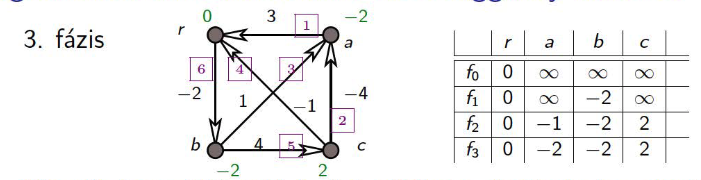
\includegraphics[width=\textwidth]{img/1.png}

        \textcolor{orange}{\textbf{Állítás:}} Ha $l$ konzervatív, akkor $dist_l(v) \forall v \in V$.

        \textcolor{green}{\textbf{Biz:}} $f_1(v) = dist_l(r,v)$ ha $\exists \leq 1$-élű legrövidebb $rv$-út. $f_2(v) = dist_l(r,v)$ ha $\exists \leq 2$-élű legrövidebb $rv$-út. $\dots$ $f_{n-1}(v) = dist_l(r,v)$ ha $\exists \leq (n-1)$-élű legrövidebb $rv$-út. Tehát $f_{n-1}(v) = dist_l(r,v) \forall v \in V$.  \textcolor{blue}{$\Box$} 

        \textcolor{orange}{\textbf{Megf:}} Ha $f_i = f_{i-1}$, akkor a Ford-algoritmust az $i$-dik fázis után be lehet fejezni, hisz nincs érdemi élmenti javítás, így $f_{n-1} = f_i$.

        \textcolor{blue}{\textbf{Megj:}} Az $f_{n-1}(v)$-t beállító élek legrövidebb utak fáját alkozják. 

        \textcolor{green}{\textbf{Biz:}} A Dijkstra esethez hasonló. Tetszőleges $v$ csúcsból visszafelé követve a végső értékeket beállító éleket $f_{n-1}(v)$ hosszúságú $rv$-utat találunk.  \textcolor{blue}{$\Box$} 

        \textcolor{blue}{\textbf{"Lépésszámanalízis":}} Ha a $|V(G)| = n$ és $|E(G)| = m$, akkor minden fázisban $\leq m$ élmenti javítás, ami $konst \cdot m$ lépés. Ez összesen $\leq konst \cdot (n-1) \cdot m \leq konst \cdot n^3$ lépés, az algoritmus hatékony.

    \subsection{Legrövidebb utak konzervatív hosszfüggvény esetén 2}

        Tegyük fel, hogy $G = (V,E), l:E \rightarrow \mathbb{R}$ és $V = \{v_1, v_2, \dots,v_n\}$. Jelölje \textcolor{red}{$d^{(k)}(i,j)$} a legrövidebb olyan $v_iv_j$-út hosszát, aminek belső csúcsai csak $v_1,v_2,\dots,v_k$ lehetnek.

        \textcolor{orange}{\textbf{Megf:}} (1) $d^{(n)}(i,j) = dist_l(v_i,v_j), v_iv_j \in E \Rightarrow d^{(0)}(i,j) = l(v_i,v_j)$ (2) $d^{(0)}(i,j) = 0$, különben $d^{(0)}(i,j) = \infty$. (3) Ha $l$ konzervatív, akkor tetszőleges $i,j$ ill. $k \leq n$ esetén $d^{(k+1)}(i,j) = min \{d^{(k)}(i,j), d^{(k)}(i,k+1)+d^{(k)}(k+1,j)\}$ teljesül.

        \textcolor{green}{\textbf{Biz:}} Tekintsünk egy $d^{(k+1)}(i,j)$-t meghatározó $P$ utat. 
        
        \textbf{I. eset:} $v_{k+1} \notin P$. Ekkor $d^{(k+1)}(i,j) = d^{(k)}(i,j)$, és $d^{(k+1)}(i,j) \leq d^{(k)}(i,k+1)+d^{(k)}(i,k+1)+d^{(k)}(k+1,j)$.

        \textbf{II. eset:} $v_{k+1} \in P$. Ekkor $d^{(k+1)}(i,j) \leq d^{(k)}(i,j)$, és $d^{(k+1)}(i,j) = d^{(k)}(i,k+1) + d^{(k)}(k+1,j)$.

        Mindkét esetben helyes a képlet.  \textcolor{blue}{$\Box$} 

        \textcolor{blue}{\textbf{Floyd-algoritmus:}} \underline{Input:} $G = (V,E)$, konzervatív $l:E \rightarrow \mathbb{R}$. \underline{Output:} $dist_l(u,v)\forall u,v \in V$ \underline{Működés:} $d^{(0)}$ felírása (2) alapján. Az $i$-dik fázis: $d^{(i-1)}$-ből meghatározzuk $d^{(i)}$-t (3) alapján. OUTPUT: $d^{(n)}(u,v) = dist_l(u,v)\; \forall u,v \in V$.

        \textcolor{blue}{\textbf{"Lépésszámanalízis":}} A $d^{(0)}$ felírása $konst \cdot n^2$ lépés. Minden fázis $konst' \cdot n^2$. Mivel összesen $n$ fázis van, a lépésszám legfeljebb $konst" \cdot n^3$ lépés, az algoritmus hatékony.

        \textcolor{orange}{\textbf{Ford vs Floyd:}} Konzervatív hosszfüggvényre működnek helyesen. Mindkét algoritmus talál bizonítékot, ha $l$ nem konzervatív. (!!) A Ford csak egy gyökérből, a Floyd bármely két csúcs között talál legrövidebb utat. (!!) A Ford ritka gráfokra jelentősen olcsóbb, sok él eletén a Floyd nem sokkal drágább.

    \subsection{Depth First Search (DFS)}

        \textcolor{blue}{\textbf{"Mélységi bejárás (DFS):}} A bejárás során mindig a legutolsónak elért csúcsot választjuk az $\boxed{1.}$ esetben.

        \textcolor{red}{Mélységi és befejezési számozás:} DFS után \textcolor{yellow}{$m(v)$} ill. \textcolor{violet}{$b(v)$} a $v$ csúcs elérési ill. befejezési sorrendben kapott sorszáma.

        \textcolor{blue}{\textbf{Megj:}} A BFS konkrét megvalósításában szükség van arra, hogy az \textcolor{yellow}{elért} csúcsokat úgy tároljuk, hogy könnyű legyen kiválasztani az \textcolor{yellow}{elért} csúcsok közül a legkorábban elértet. Erre egy célszerű adatstruktúra a \textit{sor} (avagy \textit{FIFO lista}). Ha a BFS megvalósításában ezt az adatstruktúrát \textit{veremre} (más néven \textit{FIFO listára}) cseréljük, akkor a DFS egy megvalósítása adódik.

        \textcolor{orange}{\textbf{Megf:}} Tegyük fel, hogy a $G$ gráf éleit DFS után osztályoztuk. 
        
        (1) Ha $uv$ \textcolor{green}{faél}, akkor \textcolor{yellow}{$m(u)$} $<$ \textcolor{yellow}{$m(v)$} és \textcolor{violet}{$b(u)$} $>$ \textcolor{violet}{$b(v)$}.

        \textcolor{green}{\textbf{Biz:}} $v$-t $u$-ból értük el, ezért \textcolor{yellow}{$m(u)$} $<$ \textcolor{yellow}{$m(v)$}. A $v$ elérésekor $u$ és $v$ elért állapotúak. A DFS szerint $v$-t $u$ elptt fejezzük be.  \textcolor{blue}{$\Box$} 

        (2) Ha $uv$ \textcolor{brown}{előreél}, akkor \textcolor{yellow}{$m(u)$} $<$ \textcolor{yellow}{$m(v)$} és \textcolor{violet}{$b(u)$} $>$ \textcolor{violet}{$b(v)$}.

        \textcolor{green}{\textbf{Biz:}} $u$-ból $v$-be faéleken keresztül vezet irányított út. (1) miatt az út mentén a mélységi szám növekszik, befejezési csökken.  \textcolor{blue}{$\Box$}

        (3) Ha $uv$ \textcolor{blue}{visszaél}, akkor \textcolor{yellow}{$m(u)$} $>$ \textcolor{yellow}{$m(v)$} és \textcolor{violet}{$b(u)$} $<$ \textcolor{violet}{$b(v)$}.

        \textcolor{green}{\textbf{Biz:}} $v$-ből $u$-ba faéleken keresztül vezet irányított út. (1) miatt az út mentén a mélységi szám növekszik, a befejezési csökken.  \textcolor{blue}{$\Box$}

        \textcolor{green}{\textbf{Biz:}} \textcolor{yellow}{$m(u)$} $<$ \textcolor{yellow}{$m(v)$} esetén a DFS miatt $v$ az $u$ leszármazottja lenne. Ezért $m(u) > m(u)$. Ha $u$-t a $v$ befejezése előtt érnénk el, akkor $u$ a $v$ leszármazottja lenne. Ezért az alábbi sorrendben történik $u$ és $v$ evolúciója: \textcolor{yellow}{v elérése}, \textcolor{violet}{v befejezése}, \textcolor{yellow}{u elérése}, \textcolor{violet}{u befejezése}.  \textcolor{blue}{$\Box$}
        (4) Ha $uv$ \textcolor{red}{keresztél}, akkor \textcolor{yellow}{$m(u)$} $>$ \textcolor{yellow}{$m(v)$} és \textcolor{violet}{$b(u)$} $>$ \textcolor{violet}{$b(v)$}.

        (5) Irányítatlan gráf DFS bejárása után nincs keresztél.

        \textcolor{green}{\textbf{Biz:}} Indirekt. Ha $uv$ keresztél, akkor (4) miatt \textcolor{yellow}{$m(u)$} $>$ \textcolor{yellow}{$m(v)$}, továbbá $vu$ is keresztél, ezért \textcolor{yellow}{$m(v)$} $>$ \textcolor{yellow}{$m(u)$}. Ellentmondás.  \textcolor{blue}{$\Box$}

        (6) Ha DFS után van visszaél, akkor $G$ tartalmaz irányított kört.

        \textcolor{green}{\textbf{Biz:}} A DFS fa visszaélhez tartozó alapköre a $G$ egy irányított köre.  \textcolor{blue}{$\Box$}

        (7) Ha DFS után nincs visszaél, akkor $G$-ben nincs irányított kör.

        \textcolor{green}{\textbf{Biz:}} Bmely irányított körnek van olyan $uv$ éle, amire \textcolor{violet}{$b(u)$} $<$ \textcolor{violet}{$b(v)$}. Ez az él csak visszaél lehet.  \textcolor{blue}{$\Box$} 

    \subsection{Direct Acyclic Graphs}

        \textcolor{blue}{\textbf{Def:}} A $G = (V,E)$ irányított gráf \textcolor{red}{aciklikus} (más néven \textcolor{red}{DAG}), ha $G$ nem tartalmaz irányított kört.

        \textcolor{violet}{\textbf{Példa:}} DAG-ot úgy kaphatunk, hogy egy $G$ irányítatlan gráf csúcsait csupa különbözőszámmal megszámozzuk, és minden élt a kisebb számot viselő csúcsból a nagyobba irányítunk.

        Ha ugyanis lenne az így megirányított gráfban irányított kör, akkor az élei mentén a számok végig növekednének, ami lehetetlen. Azt fogjuk ihazolni, hogy a fenti példa minden DAG-ot leír.

        \textcolor{blue}{\textbf{Def:}} A $G = (V,E)$ irányított gráf csúcsainak \textcolor{red}{topologikus sorrendje} alatt a csúcsok olyan sorrendjét értjük, amire igaz, hogy minden irányított él a sorban előbb álló csúcsból vezet a sorban későbbi csúcsba. $(V=\{v_1,v_2,\dots,v_n\},v_iv_j \in E \Rightarrow i < j)$

        \textcolor{orange}{\textbf{Tétel:}} ($G$ irányított gráf DAG) $\Leftrightarrow$ ($V(G)$-nek $\exists$ topologikus sorrendje).

        \textcolor{green}{\textbf{Biz:}} Tegyük fel, hogy $\exists$ toplogikus sorrend. Láttuk, hogy $G$ ekkor DAG. \checkmark

        \textcolor{green}{\textbf{Biz:}} Most tegyük fel, hogy $G$ DAG, és futtassunk rajra egy DFS-t. Láttuk, hogy a DFS után nem lesz visszaél, ezért minden $uv$ irányított élre $b(u) > b(v)$ teljesül. Ezért a csúcsok befejezési sorrendjének megfordítása a $G$ csúcsainak egy topologikus sorrendje.  \textcolor{blue}{$\Box$} 

        \textcolor{orange}{\textbf{Köv:}} Irányított gráf aciklikussága DFS-sel gyorsan eldönthető: ha van visszaél, akkor a visszaél DFS-fabeli alapköre $G$ egy irányított köre, így $G$ nem DAG. Ha pedig nincs visszaél, akkor a fordított befejezési sorrend a $G$ egy topologikus sorrendje, $G$ tehát DAG.

        \textcolor{blue}{\textbf{Megj:}} DAG-ban topologikus sorrendet forráskeresések és forrástörlések alkalmazásával is találhatunk.

    \subsection{Leghosszabb út keresése}

        \textcolor{violet}{\textbf{Ötlet:}} Az $l'(uv) = -l(uv)$ élhosszokkal a leghosszabb utak legrövidebbekké válnak. Olyanokat pedig tudunk keresni.

        \textcolor{red}{\textbf{Gond:}} A módszerünk csak konzervatív élhosszokra működik. Irányítatlan gráfon ez nemnegatív élhosszokat jelent, ezért ez az ötlet itt nem segít. Itányított esetben nem baj a negatív élhossz, feltéve, hogy $G$ DAG. Ekkor Ford, Floyd bármelyike használható.

        \textcolor{green}{\textbf{Jó hír:}} Van egy még gyorsabb módszer: a dinamikus programozás. Ennek segítségével tetszőleges $G$ DAG minden $v$ csúcsához ki tudjuk számítani a $v$-be vezető leghosszabb utat. (Sőt! \dots)

        \textcolor{blue}{\textbf{Leghosszabb út DAG-ban:}} \underline{Input:} $G = (V,E) DAG, l:E \rightarrow \mathbb{R}. \underline{Output:} max$\{$l(P):P v$-be vezető út\} minden $v \in V$ csúcsra. \underline{Működés:} $\boxed{1} V = \{v_1,v_2,\dots,v_n\}$ topologikus sorrend meghatározása. $\boxed{2} i = 1,2,\dots,n: f(v_i) = max\{max\{f(v_j)+l(v_jv_i):v_jv_i \in E\},0\}$ Output: $f(v)\; \forall v \in V$

        \textcolor{violet}{\textbf{Helyesség:}} Ha a $v_i$-be veeztő leghosszabb út utolsó előtti csúcsa $v_j$, akkor $f(v_i) = f(f_j) + l(v_jv_i)$.

        \textcolor{blue}{\textbf{Megj:}} Ha a fenti algoritmusban minden csúcsra megjelöljük az $f(v)$ értéket beállító élt (éleket), akkor a megjelölt élek minden $v$ csúcsba megadnak egy leghosszabb utat. Sőt: minden $v$-be vezető leghosszabb megkapható így.

    \subsection{A PERT probléma}

        Egy $a,b,\dots$ tevékenységekből álló projektet kell végrehajtanunk. 

        \textbf{Precedeniafeltételek:} bizonyos $(u,v)$ párok esetén előírás, hogy az $u$ tevékenységet a $v$ előtt kell elvégezni, ezért $v$ az $u$ kezdetét követően $c(uv)$ időkorlát elteltável kezdhető.

        \textbf{Cél:} minden $v$ tevékenységhez olyan $k(v) \geq 0$ kezdési időpont meghatározása, ami nem sérti a preferenciafeltételeket, és a projekt végrehajtási ideje (a legnagyobb $k(v)$ érték) minimális.

        G \textbf{irányított gráf} csúcsai a tevékenységek, élei pedig a precedenciafeltételek, az $uv$ él hossza $c(uv)$.

        \textcolor{orange}{\textbf{Megf:}} (1) Ha $G$ nem DAG, akkor a projekt nem hajtható végre. (2) Ha $G$ DAG, akkor minden $v$ tevékenység legkorábbi kezdási időpontja a $v$-be vezető leghosszabb út hossza.

        \textcolor{orange}{\textbf{Köv:}} A PERT probléma megoldása nem més, mint a $G$ DAG minden csúcsára az oda vezető leghosszabb út meghatározása.

        \textcolor{violet}{\textbf{Terminológia:}} $G$ leghosszabb útja \textcolor{red}{kritikus út}, amivől több is lehet. Kritikus út csúcsai a \textcolor{red}{kritikus tevékenységek.}

        \textcolor{orange}{\textbf{Megf:}} Ha egy kritikus tevékenység nem kezdődik el a lehető legkorábbi időpontban, akkor az egész projekt végrehajtása csúszik.

\end{document}